\documentclass{article}

\usepackage[swedish]{babel}
\usepackage[utf8]{inputenc}
\usepackage{amsmath}
\usepackage{hyperref}
\usepackage{underscore}
\usepackage{tikz}
\usepackage{tkz-euclide}
\usepackage{tikz-3dplot}
\usepackage{amsfonts}
\usepackage{mathtools}
\usepackage{enumitem}
\usepackage{blkarray}
\usepackage{xcolor}
\usepackage{amssymb}
\usepackage{siunitx}

\usetkzobj{all}

\DeclarePairedDelimiter \abs{\lvert}{\rvert}
\DeclarePairedDelimiter \norm{\lVert}{\rVert}

\hypersetup{
	pdfauthor={Adnan Avdagic},
	pdftitle={TATA69 Föreläsningar},
	colorlinks}

\begin{document}
\numberwithin{equation}{section}

\title{TATA69 Föreläsningar}
\author{Adnan Avdagic\\
	Linköpings Universitet\\
	\texttt{adnan@avdagic.net}}
\date{\today}
\maketitle

\newpage

\tableofcontents

\newpage
\section{Abstract}

\newpage
\noindent
\section{Föreläsning 2}
\subsection{Gränsvärden för flervarre}

\paragraph{Exempel 1} \flushleft
\begin{equation} \label{eq:1}
	f(x,y) = \frac{\sin(x^4+y^2)}{x^4+y^2} \text{, ej definierad i origo}
\end{equation}

Vad händer då (x,y) närmar sig (0,0)?

$$\lim_{x,y \rightarrow 0,0} \frac{\sin(x^4+y^2)}{x^4+y^2}$$

//sätt $t= \displaystyle x^4+y^2$, ${t \rightarrow 0}$ då ${(x,y) \rightarrow (0,0)}$// \newline
då fås \(\displaystyle \lim_{t \rightarrow 0} \frac{\sin t}{t} = 1,\) (standard gränsvärde) \newline

\paragraph{Exempel 2} \flushleft
\begin{equation} \label{eq:2}
	f(x,y) = \frac{x^3+xy}{x^2+y^2} \text{, ej definierad i origo}
\end{equation}

Gå mot origo via x-axeln (där $y=0$)
\[f(x,0) = \frac{x^3+0*x}{x^2+0^2} = \frac{x^3}{x^2} =  {x \rightarrow 0} \text{ då } {x \rightarrow 0}\]

Gå mot origo via y-axeln (där $x=0$)
\[f(0,y) = \frac{0^3+0*y}{0^2+y^2} = \frac{0}{y^2} =  {0 \rightarrow 0} \text{ då } {y \rightarrow 0}\]

Gå mot origo längs $y=x$
\[f(x,x) = \frac{x^3+x*x}{x^2+x^2} = {\frac{x+1}{2} \rightarrow \frac{1}{2}} \text{ då } {x \rightarrow 0}\]

Olika värden från olika riktningar \newline
Innanför varje liten cirkel kring origo har f värden nära 0 och nära $\frac{1}{2}$.
Vi säger därför att gränsvärde ej existerar. Se \ref{fig:1}

\begin{figure}[ht] 
\begin{tikzpicture}
   \tkzInit[xmax=5,ymax=5,xmin=-5,ymin=-5]
   \tkzAxeXY
   \draw[red,thick] (-5,0) -- (5,0);
   \draw[blue,thick] (0,-5) -- (0,5);
   \draw[green,thick] (-5,-2) -- (5,3);
   \node[above,red] at (-4,0) {\(f=x\)};
   \node[right,blue] at (0,5) {\(f=0\)};
   \node[left,green] at (3,3) {\(f=\frac{x+1}{2}\)};
   \tkzDefPoint(0,0){O}
   \tkzDefPoint(0.2,0.2){A}
   \tkzDrawCircle(O,A)
  \end{tikzpicture}
  \caption{Graf i 2D} \label{fig:1}
\end{figure}

\newpage
\subsubsection{Definition}

Funktionen \(\bar{f}\) av typ \(\mathbb{R}^n \rightarrow \mathbb{R}^m\) har gränsvärdet \(\bar{b} \in \mathbb{R}^m\) då \(\bar{x} \rightarrow \bar{a} \in \mathbb{R}^n\) om \(\forall \epsilon >0 \quad \exists \delta >0\) så att \(|\bar{f}(x)-\bar{b}|<\epsilon\) om \(0<|\bar{x}-\bar{a}|<\delta\) och \(\bar{x}\in D_f\). 
Skrivs 
\[
\lim_{\bar{x} \rightarrow \bar{a}} \bar{f}(\bar{x})=\bar{b}
\]

\newpage
\paragraph{Exempel 3}
\begin{equation} \label{eq:3}
	f(x,y)=\frac{x^3}{x^2+y^2} \text{, ej definierad i origo}
\end{equation}

\[
\begin{split}
0 \leq \abs{f(x,y)} = \frac{\abs{x^3}}{x^2+y^2} = \abs{x}\frac{x^2}{x^2+y^2} \leq \abs{x} \rightarrow 0 \text{ då } (x,y) \rightarrow (0,0) \\
\Rightarrow f(x,y) \rightarrow (0,0) \text{ då } (x,y) \rightarrow (0,0)
\end{split}
\]

Vanliga räkneregler för gränsvärden (summa, produkt, instängning) gäller också för flervarregränsvärden
Undersökning/beräkning av gränsvärden

\begin{itemize}
\item Om test av värden längs olika riktningar eller olika kurvor ger olika resultat så saknas gränsvärde, se \eqref{eq:2}
\item Sådana test kan \underline{INTE} visa att gränsvärde existerar, andra metoder behövs, som \eqref{eq:1} eller \eqref{eq:3}, eller polära koordinater
\end{itemize}

\begin{figure}[ht] 
\begin{tikzpicture}
   \tkzInit[xmax=4,ymax=4,xmin=0,ymin=0]
   \tkzAxeXY
   \tkzDefPoint(3,3){P} \tkzDefPoint(0,0){O}
   \tkzDefPoint(3,0){a} \tkzDefPoint(0,3){b} \tkzDefPoint(1.5,0){c}
   \tkzDrawArc[color=red](O,c)(P)
   \tkzDrawPoints(P)
   \tkzDrawSegment[blue](O,P)
   \tkzDrawSegment[dashed](a,P)
   \tkzDrawSegment[dashed](b,P)
   \node[right,red] at (1.5,0.5) {$\varphi$};
   \node[above left,blue] at (1.5,1.5) {$\rho$};
   \node[above right] at (3,3) {(x,y)};
  \end{tikzpicture}
  \caption{Graf för polära koordinater} \label{fig:2}
\end{figure}

\[
	\def\arraystretch{1.1}
	\begin{blockarray}{r@{\;}l}
	\begin{block}{r@{\;}l\}}
		x & = \rho \cos(\varphi) \\[\jot]
		y & = \rho \sin(\varphi) \\[\jot]
	\end{block}
	\rho  & = \sqrt{x^2+y^2} \text{, } \rho > 0 \\ [\jot]
	\tan{\varphi} & = \frac{y}{x} \text{, } 0 \leq \varphi \leq 2\pi
	\end{blockarray}
\]
Viktigt för gränsvärden: \( (x,y) \rightarrow (0,0) \iff \rho \rightarrow 0 \)

\newpage

\paragraph{Exempel \eqref{eq:3} med polära koordinater}

\[
	\lim_{(x,y) \rightarrow (0,0)} \frac{x^3}{x^2+y^2} \overset{\mathrm{pol.koord}}{=} \lim_{\rho \rightarrow 0} \frac{\rho^3\cos^3(\varphi)}{\rho^2} = \lim_{\rho \rightarrow 0} \overbrace{\rho}^{\rightarrow 0}\underbrace{\cos^3(\varphi)}_\text{begränsad} = 0
\]

\paragraph{Exempel \eqref{eq:2} med polära koordinater}

\[
\begin{split}
\lim_{(x,y) \rightarrow 0} \frac{x^3+xy}{x^2+y^2} \overset{\mathrm{pol.koord}}{=} \lim_{\rho \rightarrow 0} \frac{\rho^3 \cos^3(\varphi) + \rho^2 \cos(\varphi) \sin(\varphi)}{\rho^2} = \\
=\lim_{\rho \rightarrow 0} (\overbrace{\rho \cos^3(\varphi)}^{\rightarrow 0}+\underbrace{\cos(\varphi) \sin(\varphi)}_\text{vinkelberoende}) \Rightarrow \text{gränsvärde existerar ej}
\end{split}
\]

\subsubsection{Oändlighet i envarre och flervarre}
\subsubsection*{Envarre}
x kan gå mot $\pm\infty$
\subsubsection*{Flervarre}
bara en $\infty$ nämligen $\abs{\bar{x}} \rightarrow \infty$
\subsubsection*{2D polära}
$\abs{\bar{x}} \rightarrow \infty \iff \rho \rightarrow \infty$
\subsubsection{Definition}
\[
	\bar{f}(\bar{x}) \rightarrow \bar{b} \text{ då } \abs{\bar{x}} \rightarrow \infty \text{ om } \forall \epsilon > 0 \quad \exists \omega \text{ så att } \abs{\bar{f}(\bar{x}) - \bar{b}} < \epsilon \text{ om } \abs{\bar{x}} > \omega
\]

\newpage
\paragraph{Exempel 4}

\begin{equation} \label{eq:4}
	\lim_{(x,y) \rightarrow \infty} \frac{y}{x^2+y^2} \overset{\mathrm{pol.koord}}{=} \lim_{\rho \rightarrow \infty} \frac{\rho \sin(\varphi)}{\rho^2} = \lim_{\rho \rightarrow \infty} \overbrace{\frac{1}{\rho}}^{\rightarrow 0} \underbrace{\sin(\varphi)}_\text{Begränsad} = 0
\end{equation}

\underline{OBS!} 2-variabelfunktioner som uttryckta i polärakoordinater inte beror på $\varphi$ har rotationssymmetriska grafer kring z-axeln

\begin{figure}[ht]
\usetikzlibrary{3d}
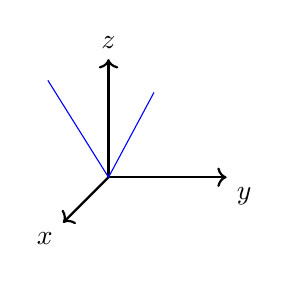
\begin{tikzpicture}
\draw[thick,->] (0,0,0) -- (0,0,1.5) node[anchor=north east]{$x$};
\draw[thick,->] (0,0,0) -- (1.5,0,0) node[anchor=north west]{$y$};
\draw[thick,->] (0,0,0) -- (0,1.5,0) node[anchor=south]{$z$};
\foreach \p in {1,...,360} {
	\draw[red] ({sin(45)*sin(\p)},{cos(45)},{sin(45)*cos(\p)}) -- ({sin(45)*sin(\p)},{cos(45)},{sin(45)*cos(\p)});
}
\draw[blue] (0,0,0) -- (0,2,2);
\draw[blue] (0,0,0) -- (0,0.5,-1.5);
\end{tikzpicture}
\caption{Exempel på rotationssymmetri} \label{fig:3}
\end{figure}

\(
z = \sqrt{x^2+y^2} = \rho
\)

\subsubsection{3-variabler mot origo}
\paragraph{Exempel 5}

\begin{equation}
	\lim_{(x,y,z) \rightarrow (0,0,0)} \frac{xyz}{x^2+y^2+2z^2} = \text{ ???}
\end{equation}

\[
	0 \leq \abs{\frac{xyz}{x^2+y^2+2z^2}} = \frac{\abs{x}\abs{y}\abs{z}}{x^2+y^2+2z^2} \leq \frac{\abs{x}\abs{y}\abs{z}}{x^2+y^2+z^2} \leq 
\]

\[
	// 
	\def\arraystretch{1.1}
	\begin{blockarray}{r@{\;}l}
	\abs{x} \leq \sqrt{x^2+y^2+z^2} \\ [\jot]
	\abs{y} \leq \sqrt{x^2+y^2+z^2} \\ [\jot]
	\abs{z} \leq \sqrt{x^2+y^2+z^2}
	\end{blockarray}
	//
\]

\[
\begin{split}
	\leq \frac{\sqrt{x^2+y^2+z^2}}{x^2+y^2+z^2} = \sqrt{x^2+y^2+z^2} \rightarrow 0 \text{ då } (x,y,z) \rightarrow (0,0,0) \\
	\Rightarrow \lim_{(x,y,z) \rightarrow (0,0,0)} \frac{xyz}{x^2+y^2+2z^2} = 0
\end{split}
\]

\newpage
\subsection{Rymdpolära koordinater}

\begin{figure}[ht]
\usetikzlibrary{3d}
\begin{tikzpicture}
\draw[thick,->] (0,0,0) -- (0,0,5) node[anchor=north east]{$x$};
\draw[thick,->] (0,0,0) -- (5,0,0) node[anchor=north west]{$y$};
\draw[thick,->] (0,0,0) -- (0,5,0) node[anchor=south]{$z$};
\draw[dashed]
	(0,4,0) --
	(4,4,4) coordinate (p) --
	(4,0,4) coordinate (q);
\draw[thick,red]
	(0,0,0) coordinate (o)-- (q);
\draw[dashed] 
	(0,0,4) coordinate (x) -- (q) -- (4,0,0);
\draw[thick,blue] (o) -- (p);
\draw[green] let
	\p0 = (o),
	\p1 = (0,0,2),
	\p2 = (2,0,2),
	\n1 = {atan2(\p1)},
    \n2 = {\n1 + 103},
    \n3 = {1cm},
    \n4 = {(\n1 + \n2) / 2}
  in (o) +(\n1:\n3) arc[radius = \n3, start angle = \n1, end angle = \n2];
\draw[purple] let
	\p0 = (o),
	\p1 = (0,0,2),
	\p2 = (2,0,2),
	\n1 = {atan2(2,0)},
    \n2 = {atan2(2,2)},
    \n3 = {1cm},
    \n4 = {(\n1 + \n2) / 2}
  in (o) +(\n1:\n3) arc[radius = \n3, start angle = \n1, end angle = \n2];
\node[fill,circle,inner sep=1.5pt,label={above right:$(x,y,z)$}] at (p) {};
\node[left,blue] at (2,2,2) {$r$};
\node[right,red] at (1,0,1) {$r\sin(\theta)$};
\node[above,green] at (1,0,2.5) {$\varphi$};
\node[above left,purple] at (0.7,1,0) {$\theta$};
\end{tikzpicture}
\caption{Rymdpolära koordinater} \label{fig:4}
\end{figure}

\[
\left\{\begin{array}{rcl}
	x & = r \sin(\theta) \cos(\varphi) \\
	y & = r \sin(\theta) \sin(\varphi) \\
	z & = r \cos(\theta) 
\end{array}\right.
\]
\[
\begin{split}
	r & = \sqrt{x^2+y^2+z^2} \text{, } r > 0 \\
	0 & \leq \theta \leq \pi \\
	r & \sin(\theta) = \rho
\end{split}
\]

För gränsvärden där \((x,y,z) \rightarrow (0,0,0) \iff r \rightarrow 0\)

\newpage
\paragraph{Exempel 5 med rymdpolära koordinater}

\[
\begin{split}
	\lim_{(x,y,z) \rightarrow (0,0,0)} \frac{xyz}{x^2+y^2+2z^2} \overset{\mathrm{rymdpol.koord}}{=} \\
	= \lim_{r \rightarrow 0} \frac{r^3 \sin^2(\theta) \cos(\theta) \sin(\varphi) \cos(\varphi)}{r^2+r^2 \cos^2(\theta)} = \\
	= \lim_{r \rightarrow 0} \overbrace{r}^{\rightarrow 0} \underbrace{\frac{\sin^2(\theta) \cos(\theta) \sin(\varphi) \cos(\varphi)}{1+\cos^2(\theta)}}_\text{begränsad, nämnare \(\geq 1 \) ingen risk för /0}
\end{split}
\]

\subsubsection{Cylindriska koordinater}

Polära koordinater i (x,y) och vanliga i z

\[
\left\{\begin{array}{rcl}
	x & = r \cos(\varphi) \\
	y & = r \sin(\varphi) \\
	z & = z 
\end{array}\right.
\]

\newpage
\section{Föreläsning 3}
\subsection{Partiella derivator}

\paragraph{Exempel 1}

\begin{equation} \label{eq:3.1}
	f(x,y) = x^2y + x\sin(y)
\end{equation}

Hur förändras \(f\) om bara \(x\) varieras? Vi vill derivera \(f\) m.a.p \(x\) och hålla \(y\) konstant. Skrivs:

\[
	\underbrace{f^{\prime}_{x}(x,y) = \frac{\partial f}{\partial x}(x,y)}_{\text{båda skrivsätten används}} = 2xy+\sin(y)
\]

Motsvarande då bara \(y\) varieras

\[
	f^{\prime}_{y}(x,y) = \frac{\partial f}{\partial y}(x,y) = x^2 + x\cos(y)
\]

\subsubsection{Definition}

Partiella derivatan av \(f(x,y)\) m.a.p \(x\) i punkten \((x,y)\) är

\[
	f^{\prime}_{x}(x,y) = \lim_{h \rightarrow 0} \frac{f(x+h,y) - f(x,y)}{h}
\]

Om gränsvärde existerar! \newline

Motsvarande för y:

\[
	f^{\prime}_{y}(x,y) = \lim_{k \rightarrow 0} \frac{f(x,y+k) - f(x,y)}{k}
\]

\begin{figure}[ht] 
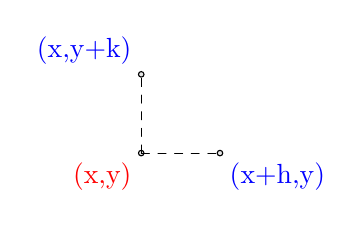
\begin{tikzpicture}
   \tkzInit[xmax=4,ymax=4,xmin=0,ymin=0]
   \tkzAxeXY
   \tkzDefPoint(2,2){a} \tkzDefPoint(3,2){b} \tkzDefPoint(2,3){c}
   \tkzDrawPoints(a,b,c)
   \tkzDrawSegment[dashed](a,b)
   \tkzDrawSegment[dashed](a,c)
   \node[below left,red] at (a) {(x,y)};
   \node[below right,blue] at (b) {(x+h,y)};
   \node[above left,blue] at (c) {(x,y+k)};
  \end{tikzpicture}
  \caption{Grafisk visning av hur f ändras i x- \& y-riktningen} \label{fig:5}
\end{figure}

\paragraph{Exempel 2}

3 variabler

\begin{align*}
\begin{split}
	f(x,y,z) = x^3y^2z+z^2e^y \Rightarrow \\
	\Rightarrow \left\{\begin{array}{rcl}
		f_{x}^{\prime}(x,y,z) = & 3x^2y^2z \\
		f_{y}^{\prime}(x,y,z) = & 2x^3yz+z^2e^y \\
		f_{z}^{\prime}(x,y,z) = & x^3y^2+2ze^y
	\end{array}\right.
\end{split}
\end{align*}

\subsubsection{Andraderivator}

\[
\begin{split}
	f_{xx}^{\prime\prime} = \frac{\partial^2f}{\partial x^2} = \frac{\partial}{\partial x} \left(\frac{\partial f}{\partial x}\right) \\
	f_{xy}^{\prime\prime} = \frac{\partial^2f}{\partial y\partial x} = \frac{\partial}{\partial y} \left(\frac{\partial f}{\partial x}\right)
\end{split}
\]

\paragraph{Exempel \eqref{eq:3.1} andra derivator}

\[
	f_{xx}^{\prime\prime} = 2y
\]
\[
\left.\begin{array}{rcl}
	f_{xy}^{\prime\prime} = 2x + \cos(y) \\
	f_{yx}^{\prime\prime} = 2x + \cos(y)\\
\end{array}\right\}\text{lika, ingen slump}
\]
\[
	f_{yy}^{\prime\prime} = -x\sin(y)
\]

Skriv \(f\in C^r\) om \(f\):s alla \(r\):te-derivator är kontinuerlig.

\subsubsection{Sats}

\[
	f \in C^2 \Rightarrow f_{xy}^{\prime\prime} = f_{yx}^{\prime\prime}
\]

motsvarande för \(\geq 3\) varianter \newline

\(f(x,y)\) har 4 andraderivator varav 3 olika \\
\(f(x,y,z)\) har 9 andraderivator varav 6 olika

\newpage

\paragraph{Exempel 3}

Bestäm alla \(f(x,y,z)\) som uppfyller

\begin{equation}
\begin{split}
	f_{x}^{\prime} = p(x,y,z) = 3x^2yz \quad (1) \\
	f_{y}^{\prime} = q(x,y,z) = x^3z + 2ye^z \quad (2) \\
	f_{z}^{\prime} = r(x,y,z) = x^3y + y^2e^z \quad (3) 
\end{split}
\end{equation}

\underline{Systematisk lösning}

\[
\begin{split}
	(1) \Rightarrow f(x,y,z) = x^3yz+\overbrace{\underbrace{g(y,z)}^{\text{godtycklig}}_{\text{2-variabel} f}} \\
	\underline{\text{Derivera detta m.a.p } y} \\
	\Rightarrow x^3z+g_{y}^{\prime}(y,z) = x^3z+2ye^z \Rightarrow \\
	\Rightarrow g_{y}^{\prime}(y,z) = 2ye^z \Rightarrow \\
	\Rightarrow g(y,z) = y^2e^z + \overbrace{\underbrace{h(z)}^{\text{godtycklig}}_{\text{envarre }f}} \Rightarrow \\
	\Rightarrow f(x,y,z) = x^3yz+y^2e^z+h(z) \\
	\underline{\text{Derivera detta m.a.p } z} \\
	\Rightarrow x^3y+y^2e^z+h^{\prime}(z) = x^3y+y^2e^z \Rightarrow \\
	\Rightarrow h^{\prime}(z) = 0 \Rightarrow h(z) = C \Rightarrow
\end{split}
\]

\[
	\Rightarrow \text{Svar: } f(x,y,z) = x^3yz+y^2e^z+C \text{ ,\(C\) är en godtycklig konstant}
\]

\centerline{Man kan visa att systemet (1) - (3) är lösbart}
\[
	\iff
\]
\[
\begin{split}
	p_{y}^{\prime} = q_{x}^{\prime} \\
	p_{z}^{\prime} = r_{x}^{\prime} \\
	q_{z}^{\prime} = r_{y}^{\prime} 
\end{split}
\]

\paragraph{Exempel 4}

\[
\begin{split}
	f_{x}^{\prime} = xy \\
	f_{y}^{\prime} = x^2 \\
	\text{olösbart ty} \\
	f_{xy}^{\prime\prime} = x \neq f_{yx}^{\prime\prime} = 2x
\end{split}
\]

\subsection{Differentierbarhet}
\subsubsection*{Envarre}

Om \(f_{a}^{\prime} = \lim_{h \rightarrow 0} \frac{f(a+h) - f(a)}{h} \quad \exists\) (dvs \(f\) deriverbar i \(a\)) så finns talet \(f_{a}^{\prime} = A\) sådant att \(\frac{f(a+h) - f(a)}{h}-A = \frac{1}{h}(f(a+h)-f(a)-Ah) = \rho(h) \rightarrow 0\) \newline \newline
Vi vet att \(f \in C^1 \Rightarrow f\) deriverbar \(\Rightarrow f\) kontinuerlig 

\subsubsection*{Flervarre}
\subsubsection{Definition}

\(f(x,y)\) är \underline{differentierbar} i \((a,b)\) om \(\exists\) tal \(A,B\) så att

\[
	\frac{1}{\sqrt{h^2+k^2}} (f(a+h,b+k) - f(a,b) - Ah - Bk) = \rho(h,k) \rightarrow 0 \text{ då } (h,k) \rightarrow (0,0)
\]

så deriverbar = differentierbar för envarre
För \(\geq\) 2 variabler gäller

\subsubsection{Sats}

\[
	f \in C^1 \overset{(1)}{\Rightarrow} f \text{ differentierbar} \left\{\begin{array}{rcl}
	\overset{(2)}{\Rightarrow} f \text{ partiellt deriverbar} \overset{(4)}{\nRightarrow} f \text{ kontinuerlig} \\
	\overset{(3)}{\Rightarrow} f \text{ kontinuerlig} \overset{(5)}{\nRightarrow} f \text{ partiellt deriverbar}
	\end{array}\right.
\]

\paragraph{Förklaring av pilar}
\begin{enumerate}
	\item s.56-57 i boken
	\item \(
				f_{x}^{\prime}(a,b) = \lim_{h \rightarrow 0} \frac{f(a+h,b) - f(a,b)}{h} \overset{f \text{ diff.bar med }k=0}{=} \lim_{h \rightarrow 0} \frac{Ah + B*0 + \sqrt{h^2 + 0^2}\rho(h,0)}{h} = \lim_{h \rightarrow 0} A \underbrace{\frac{\sqrt{h^2}}{h}}_{\pm \text{ 1 begränsad}} \underbrace{\frac{\rho(h,0)}{h}}_{\rightarrow 0} = A \quad \exists
			\)
	\item \(
				f(a+h,b+k) = f(a,b) + \underbrace{Ah}_{\rightarrow 0} + \underbrace{Bk}_{\rightarrow 0} + \underbrace{\sqrt{h^2 + k^2}}_{\rightarrow 0}\underbrace{\rho(h,k)}_{\rightarrow 0} \rightarrow f(a,b) \text{ då } (h,k) \rightarrow (0,0) \Rightarrow f \text{ kontinuerlig}
			\)
	\item Motexempel finns i boken s.51
	\item Motexempel \(f(x,y) = \abs{x}\) i \((0,0)\), kontinuerlig men \(f_{x}^{\prime}(x,y) \quad \nexists\)
\end{enumerate}

\newpage

\subsubsection{Linjär avbildning}

Den linjära avbildningen \(df_{(a,b)}\) av typ \(\mathbb{R}^2 \rightarrow \mathbb{R}\), som definieras av \(df_{(a,b)}(h,k) = Ah + Bk = f_{x(a,b)}^{\prime}h + f_{y(a,b)}^{\prime}k\), kallas \underline{differentialen} av \(f\) i (a,b) \\
ofta skrivs variablerna \(h=dx\) \& \(k=dy\) så \(df_{(a,b)}(dx,dy) = f_{x(a,b)}^{\prime}dx + f_{y(a,b)}^{\prime}dy\) eller kort \(df = f_{x}^{\prime}dx + f_{y}^{\prime}dy\)

\paragraph{Exempel \eqref{eq:3.1} omskrivet}

\[
	f(x,y) = x^2y + x\sin(y) \Rightarrow df = (2xy+\sin(y))dx + (x^2+x\cos(y))dy
\]

\subsubsection*{Feluppskattning med \(df\)}

Om \(\overline{\Delta x} = (\Delta x_{1},...,\Delta x_{n}) \in \mathbb{R}^n\) och \(f\) är differentierbar fås \(f(\overline{x} + \overline{\Delta x}) - f(\overline{x}) = f_{x_{1}}^{\prime}\Delta x_{1} + ... + f_{x_{n}}^{\prime}\Delta x_{n} + \underbrace{\rho(\Delta x_{1},...,\Delta x_{n})\sqrt{(\Delta x_{1})^2 + ... + (\Delta x_{n})^2}}_{\text{Restterm}} \approx df(\overline{\Delta x})\) 

\subsubsection*{Exempel 5}

Bestäm rörelseenergin och uppskatta felet för massan \(m = 1.0 \pm 0.1\si{\kilogram}\) med hastighet \(v = 4.0 \pm 0.2\si{\metre\per\second}\). \newline
Formel för rörelseenergi: \(E = \frac{mv^2}{2} \si{\joule}\) \newline
Utan fel: \(E = \frac{1*1.4^2}{2} = 8.0 \si{\joule}\) \newline
Fel: 
\[
\begin{split}
	\Delta E = E(m + \Delta m, v + \Delta v) - E(m,v) \approx dE(\Delta m,\Delta v) = \\
	= \frac{\partial E}{\partial m} \Delta m + \frac{\partial E}{\partial v} \Delta v = \underbrace{\frac{v^2}{2}}_{\frac{4^2}{2}} \Delta m + \underbrace{mv}_{1*4} \Delta v = 8\Delta m + 4\Delta v \\
	\Rightarrow \text{ maxfel } \leq 8\abs{\Delta m} + 4\abs{\Delta v} = 8*0.1 + 4*0.2 = 1.6 \si{\joule} \Rightarrow E = 8.0 \pm 1.6 \si{\joule}
\end{split}
\]

\newpage
\section{Appendix}
\begin{appendix}
	\listoffigures
	\listoftables
\end{appendix}

\end{document}